\section*{Fra Konserthuset til Frognerparken}

Oppgaven er basert på konseptet om komplekse tall, som er en utvidelse av de vanlige tallene vi bruker til vanlig, altså alle heltall $1, 2, -4, 7$ etc, alle rasjonale tall $\frac{2}{3}, \frac{6}{17}$ etc, og alle reelle tall $\pi, \sqrt{2}, 0.99999...$, etc. Komplekse tall er todimensjonale, som gjør at vi kan bruke de til å beskrive posisjon på et kart. Det er i hovedsak to måter å beskrive et komplekst tall på, komplekse koordinater og polarkoordinater. Den førstnevnte er tall på formen $a+bi$ og den andre er tall på formen $r\mathrm{e}^{\phi i}$, hvor $a,b,r$ er reelle tall, $i$  er den imaginære enheten $\sqrt{-1}$ og $\phi$ er en vinkel oppgitt i radianer. I oppgaven er det oppgitt at vi står i posisjon $0+0i$, og at kongen bor ved $4.61\mathrm{e}^{\theta i}$, hvor $\theta=102.53^\circ$. 

Det første vi må gjøre er å uttrykke disse to posisjonene i samme type koordinater, og vi velger i dette forslaget å bruke komplekse koordinater. Vi ser at vinkelen til posisjonen til slottet er oppgitt i grader og ikke radianer, så vi konverterer først $102.53^\circ$ om til radianer ved å multiplisere med $\frac{\pi}{180}$. Vi får da $\phi = 1.78948608$ radianer. 

Vi kan konvertere fra polarkoordinater, $r\mathrm{e}^{\phi i}$, til komplekse koordinater, $a+bi$, ved å bruke følgende formler: 

\begin{itemize}
    \item $a = r\cdot \cos(\phi)$
    \item $b=r\cdot \sin(\phi)$
\end{itemize}

Gjør vi dette med kongens koordinater får vi $-1.00014 + 4.5002 i$, som vi kan avrunde til $-1+4.5i$. Dersom vi nå lar destinasjonen vår være $x+yi$ kan vi omformulere problemet vårt til 

$$
(x+yi)\cdot \frac{1}{49}(11-7i) = -1+4.5i,
$$

som vi kan løse for $x$ og $y$. Ved å gange ut venstre side av ligningen får vi 

$$
\frac{1}{49}(11x+7y)+\frac{1}{49}(11y-7x)i = -1+4.5i
$$

som vil si at vi må løse det følgende ligningssystem med to ukjente: 

\begin{itemize}
    \item $\frac{11}{49}x+\frac{7}{49}y = -1$
    \item $\frac{11}{49}y-\frac{7}{49}x = 4.5$
\end{itemize}

Vi kan enkelt løse dette ved å først løse den øverste ligningen for $x$, som gir $x=\frac{-49-7y}{11}$. Ved å sette dette utrykket inn for $x$ i den andre ligningen, samt å løse for $y$ får vi $y=12.25$. Denne verdien kan vi igjen sette inn i første ligning, som gir $x = 12.25$. Altså er posisjonen til destinasjonen vi skal til gitt som $12.25 + 12.25i$ i komplekse koordinater. 

Vi har nå nesten alt vi trenger for å finne destinasjonen vår, det siste vi trenger er et kart over Oslo. Vi legger inn posisjonen vår og posisjonen til slottet ved $(-1,4.5)$, markert med en rosa vektor. 

\begin{center}
    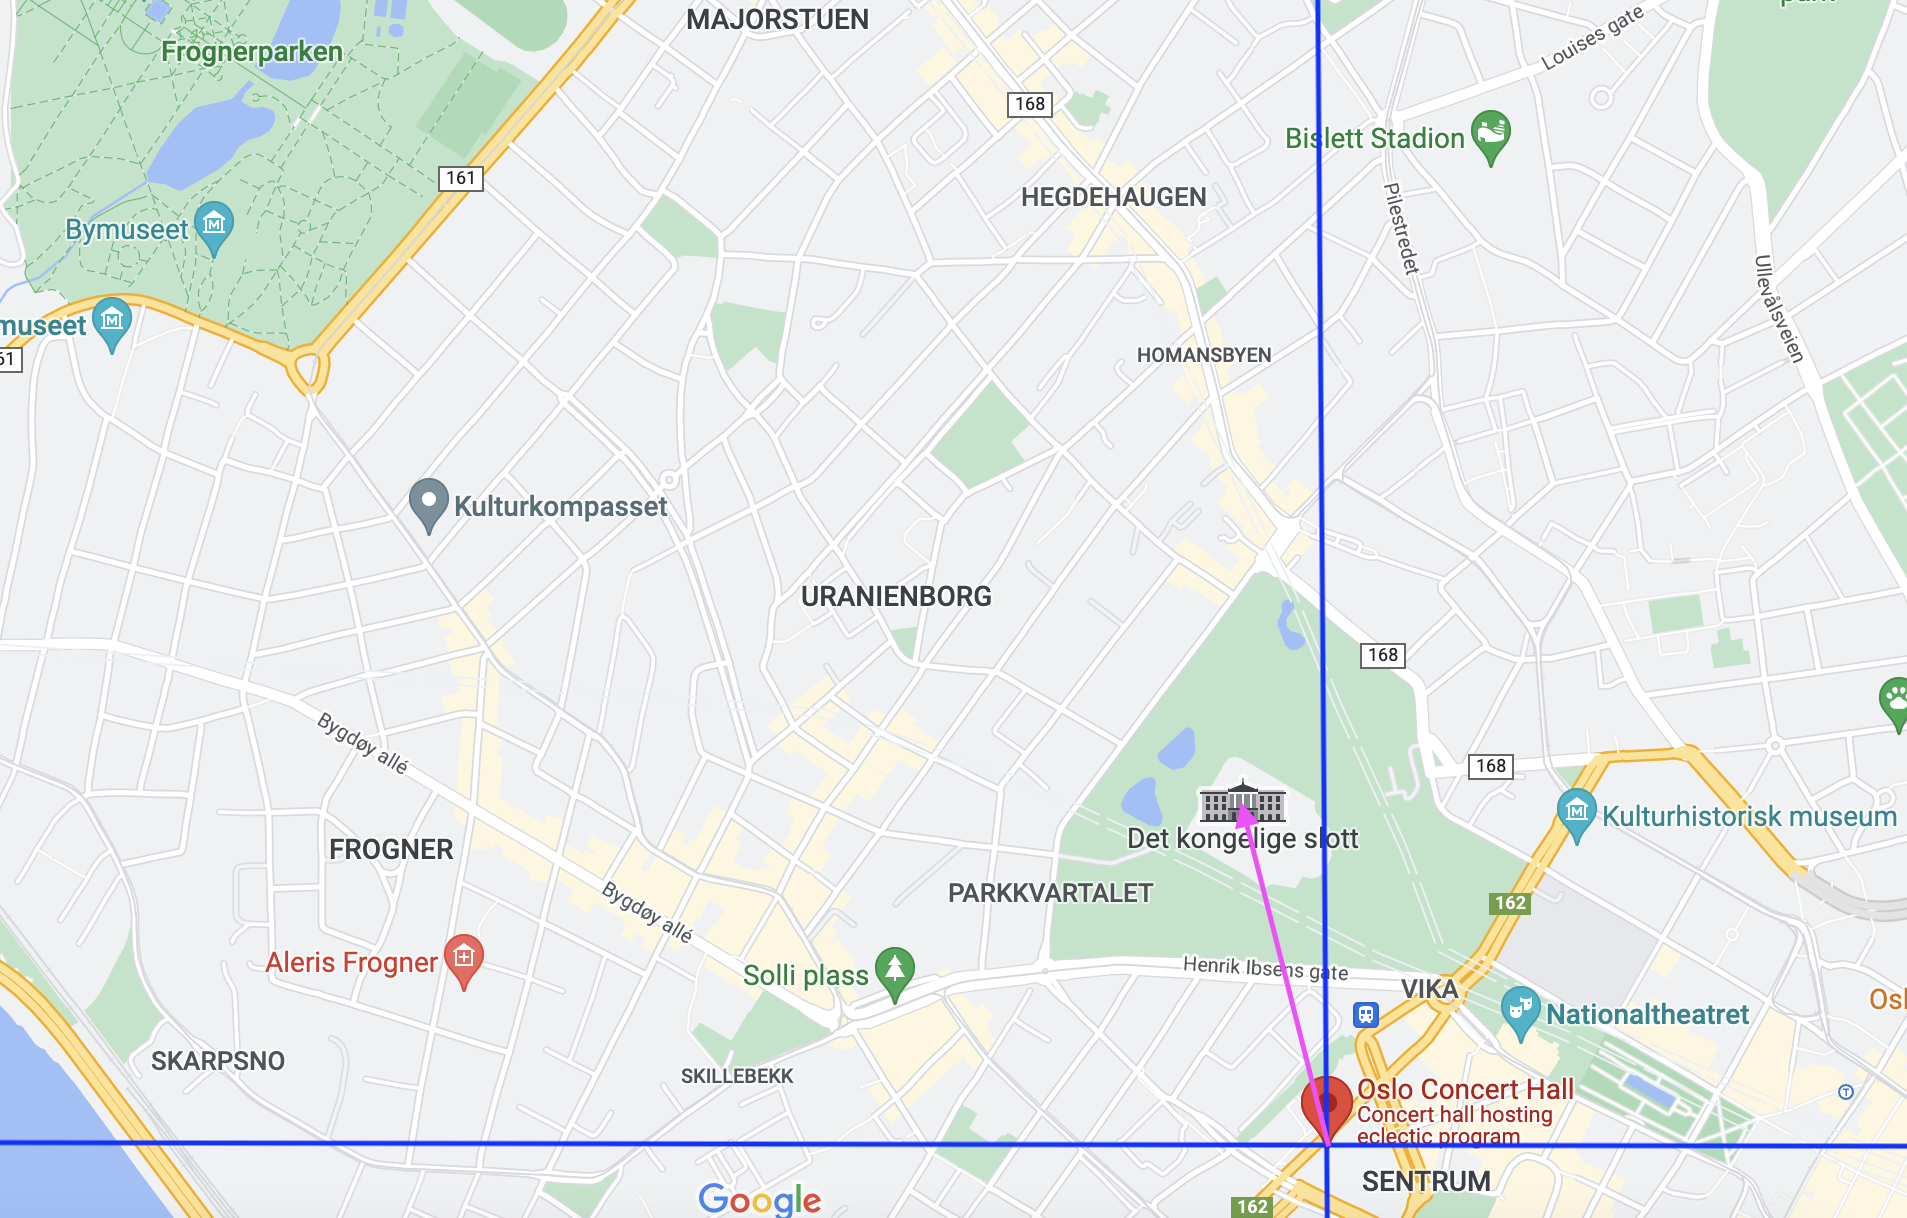
\includegraphics[width=\textwidth]{img/frogner.png}
\end{center}

Vi kan så bruke komponentene til denne vektoren til å finne destinasjonen vår. Vi får

\begin{center}
    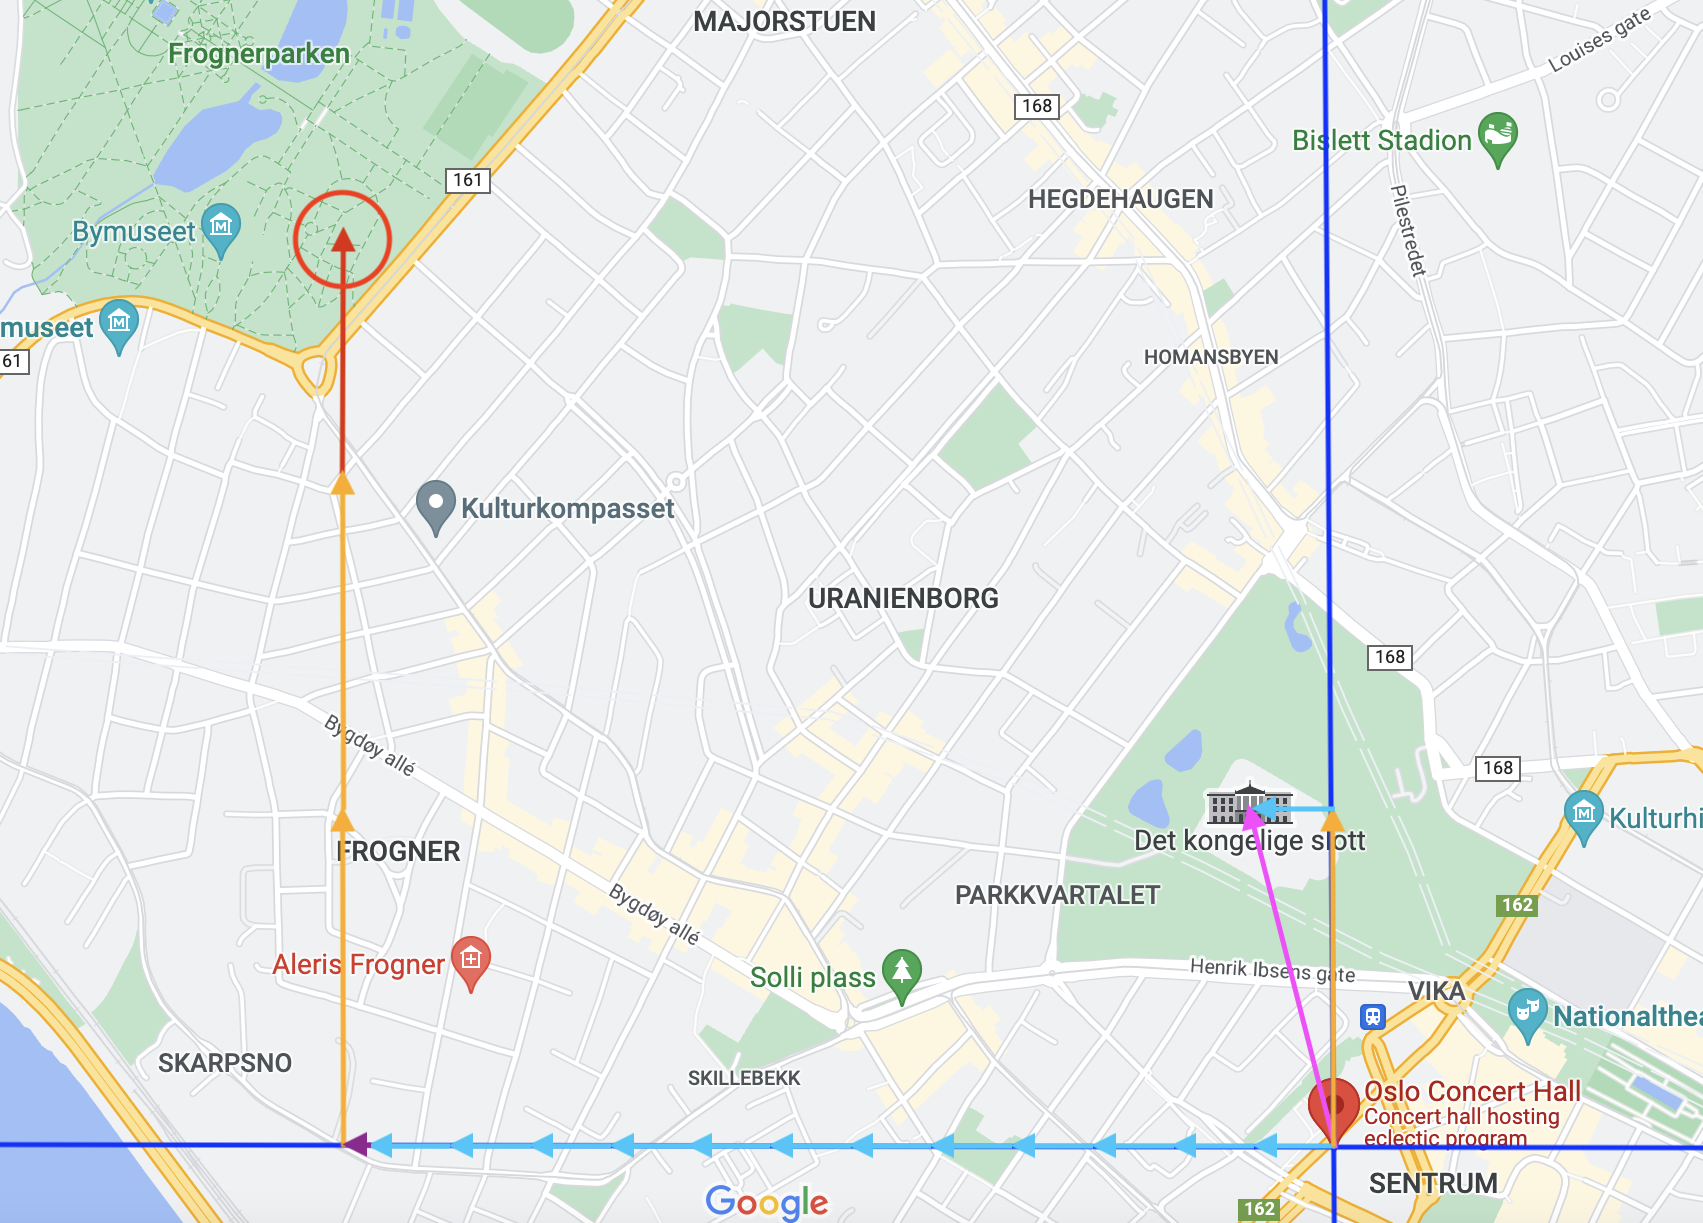
\includegraphics[width=\textwidth]{img/frogner_vec.png}
\end{center}

der de lyseblå vektorene har lengde $1$, de oransje har lengde $4.5$, den mørke blå har lengde $0.25$ og den røde har lengde $3.25$. Disse beskriver tilsammen posisjonen til destinasjonen vår $(12.25, 12.25)$. Dette viser at destinasjonen vår er Frognerparken!

